\section{ساختار تصویربرداری \mri}\label{sec:mri-basics}

\subsection{تاریخچه}


تاریخچه تصویربرداری تشدید مفناطیسی
\LTRfootnote{Magnetic Resonance Imaging}(\mri)
تلاش تعداد زیادی از محققانی را شامل می‌شود که پدیده تشدید مغناطیسی هسته
\LTRfootnote{Nuclear Magnetic Resonance}(\lr{NMR})
را کشف کردند.
در سال ۱۹۵۰، حصول تصویر یک بعدی \mri توسط هرمن کار 
\LTRfootnote{Herman Carr}
 گزارش گردید. پاول لاتربر 
\LTRfootnote{Paul C. Lauterbur}
، شیمیدان آمریکایی با کار بر روی تحقیقات پیشین، موفق به ابداع روش‌هایی برای تولید تصاویر دو بعدی و سه بعدی \mri گردید. سرانجام وی در سال ۱۹۷۳ اولین تصویر گرفته شده بر اساس تشدید مغناطیس هسته‌ای (\lr{NMR}) خود را منتشر نمود. اولین تصویر مقطع نگاری از یک موش زنده در ژانویه ۱۹۷۴ منتشر گردید.


از سوی دیگر تحقیقات و پیشرفت‌های مهمی در زمینهٔ تصویر برداری بر اساس تشدید مغناطیسی هسته برای نخستین بار در دانشگاه ناتینگهام انگلستان 
\LTRfootnote{University of Nottingham}
صورت پذیرفت، جایی که پیتر منسفیلد فیزیکدان برجستهٔ آن مؤسسه با گسترش یک روش ریاضی موفق به کاهش زمان تصویربرداری و افزایش کیفت تصاویر نسبت به روش بکارگرفته شده توسط لاتربر گردید. در همان زمان در سال ۱۹۷۱ دانشمند آمریکایی ارمنی تبار ریموند دامادیان استاد دانشگاه ایالتی نیویورک در مقاله‌ای که در مجلهٔ Science منتشر گردید، اعلام نمود که امکان تشخیص تومور از بافت‌های عادی به کمک تصویر برداری 
\lr{NMR}
 میسر می‌باشد.

سرانجام جایزهٔ نوبل پزشکی سال ۲۰۰۳ به خاطر اختراع ام آر آی به پاول لاتربر از دانشگاه ایلینوی در اوربانا شامپاین و پیتر منزفیلد از انگلستان اعطا گردید. 
این جایزه به تنهایی می‌تواند اهمیت این نوع تصویربرداری را نشان دهد.

اما چه عواملی باعث شده‌اند تا این‌قدر \mri بااهمیت و ویژه باشند؟ تصویربرداری \mri روشی غیر تهاجمی و نسبتا امن است. 

سیستم‌های ام آر آی امروزه غالباً دارای قدرت میدان‌های ۰/۲، ۱، ۱/۵، و ۳ تسلا می‌باشند.
در ایالات متحده آمریکا بیمارستان‌ها و مراکز خدمات بهداشتی اجازه استفاده از سیستم‌های تا ۴ تسلا را نیز برای یک بیمار دارند. اما از چهار تسلا به بالا صرفاً جنبه و کاربردهای تحقیقاتی دارد.

امروزه بزرگ‌ترین تولیدکننده‌های سیستم‌های ام آر آی شرکت‌های زیمنس (آلمان)، جنرال الکتریک (آمریکا)، توشیبا (ژاپن)، و فیلیپس (هلند) می‌باشند.

\subsection{خطرات \mri}
برخلاف سایر دستگاه‌های تصویربرداری مثل اشعه ایکس و سی‌تی اسکن، ام آر آی از تشعشع یونیزه استفاده نمی‌کند. از این ابزار می‌توان برای تصویربرداری از جنین در دوران بارداری استفاده کرد بدون آن که اثری روی آن داشته باشد. اما باز هم این روش ممکن است خطراتی در پی داشته باشد و به همین دلیل جوامع پزشکی استفاده از \mri را در مراحل اولیه تشخیص بیماری توصیه نمی‌کنند. از آن‌جایی که در فرآیند ام آر آی از مغناطیس قوی استفاده می‌شود هر قطعه فلزی که در بدن وجود داشته باشد مثل ضربان ساز قلب، مفصل مصنوعی، دریچه مصنوعی قلب، حلزون مصنوعی گوش و یا هر نوع صفحه و پیچ و مهره فلزی در بدن ممکن است خطرساز باشد، چون میدان مغناطیسی می‌تواند باعث جابجایی و یا گرم شدن آن قطعه شود.

تعدادی از بیمارانی که از ضربان ساز قلب استفاده می‌کردند طی انجام ام آر آی از دنیا رفتند. بنابراین لازم است تکنولوژیست \mri سوالات لازم را قبل از انجام این فرآیند از بیمار بپرسد. البته بیشتر قطعات فلزی که امروز در ایمپلنت‌های بدن استفاده قرار می‌شوند تحت تأثیر میدان‌های مغناطیسی قرار نمی‌گیرند و به اصطلاح
\lr{MR-Safe}
 هستند. علاوه بر این، هنگام اسکن، دستگاه ام آر آی صداهای بلندی تولید می‌کند که ممکن است باعث ناراحتی فرد شود، بنابراین استفاده از حفاظ گوش در طول این فرآیند ضروری است.




\begin{figure}
	\centering
%	\copyrightbox[b]{
%	\begin{minipage}[c]{0.9\textwidth}
%	\centering
	\subfigure[تصویر پاول لاتربور]{
		\copyrightbox[b]{
		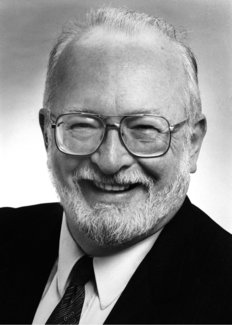
\includegraphics[height=0.36\linewidth]{mychapters/chapter-2/figs/lauterbur-13686-content-portrait-mobile-tiny}
		}{\urlSource{https://is.gd/HgbMvo}}
		\label{subfig:paullauterbur}
	}
	\hspace{0.1\linewidth}
	\subfigure[تصویر هرمن کار]{
		\copyrightbox[b]{
		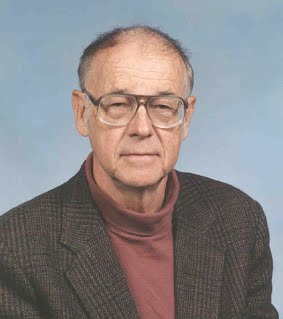
\includegraphics[height=0.36\linewidth]{mychapters/chapter-2/figs/herman_carr}
		}{\urlSource{https://is.gd/teAHxS}}
		\label{subfig:herman-carr}
	}
	\hspace{0.1\linewidth}
	\subfigure[تصویر Peter-Mansfield]{
		\copyrightbox[b]{
			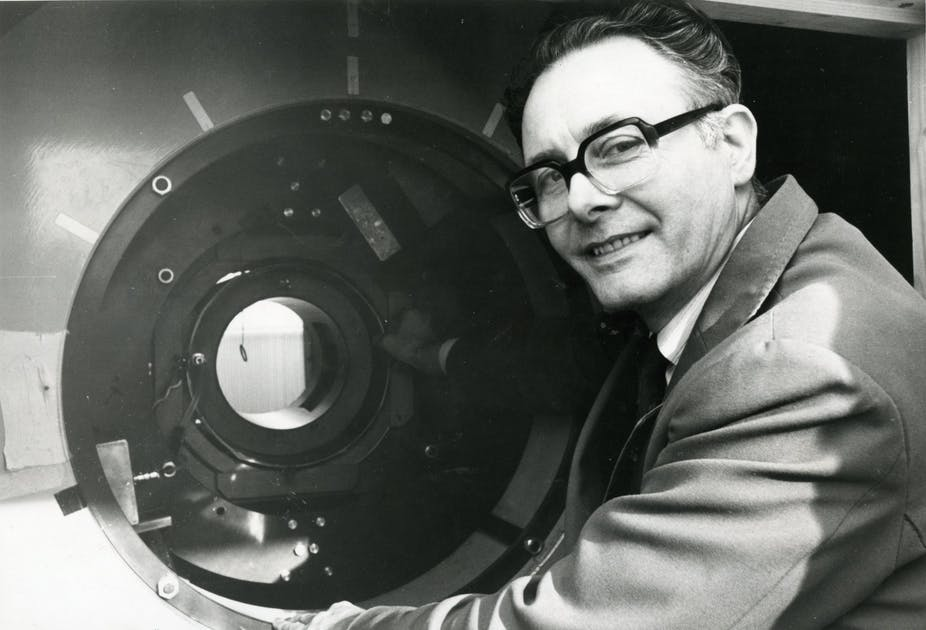
\includegraphics[height=0.36\linewidth]{mychapters/chapter-2/figs/Peter-Mansfield}
		}{\urlSource{https://is.gd/W7AXIL}}
		\label{subfig:Peter-Mansfield}
	}


%	\end{minipage}
%	}{\scriptsize\url{https://www.nobelprize.org/prizes/medicine/2003/lauterbur/biographical/}
%		\url{https://sites.google.com/a/pbsd.k12.pa.us/magnetic-resonance-imaging/herman-carr}
%		\url{https://theconversation.com/obituary-professor-sir-peter-mansfield-whose-invention-of-the-mri-scanner-revolutionised-medicine-72815}}
	\caption{تصویر سازندگان اصلی دستگاه تصویربرداری \mri}
	
	
\end{figure}



\begin{figure}
	\centering
	\copyrightbox[b]{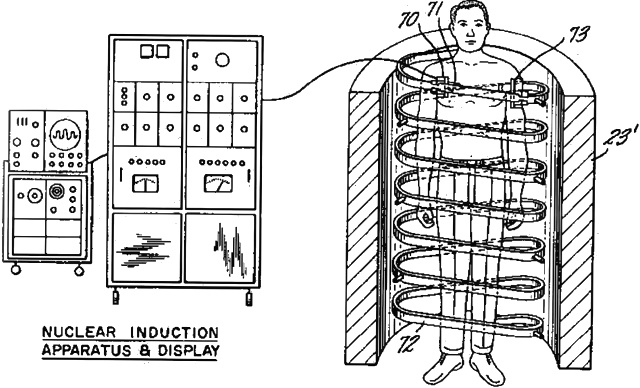
\includegraphics[width=0.6\linewidth]{mychapters/chapter-2/figs/Damadian_invention}}
	{\urlSource{https://w.wiki/3STS}}
	\caption{تصویری از آرشیو اداره ثبت اختراعات آمریکا که متعلق به ریموند دامادیان، دانشمند آمریکایی و یکی از مخترعین سیستم‌های نوین ام آر آی}
	\label{fig:Damadian_invention}
\end{figure}


\subsection{بررسی مفهوم اسپین}
 

ساختار یک اتم، یکی از اجزای اساسی در آزمایشات تشدید مغناطیسی است. اتم ها از سه ذره اصلی 
\LTRfootnote{Fundamental Particles}
تشکیلی شده اند:
\begin{enuminline}
	\item پروتون، که بار مثبت دارد
	\item نوترون، که بدون بار است
	\item الکترون، که بار الکتریکی منفی دارد
\end{enuminline}.
پروتون‌ها و نوترون‌ها در درون هسته اتم قرار گرفته اند و الکترون‌ها در خارج هسته به دور آن می‌گردند.
همچنین \textit{عدد‌اتمی}
\LTRfootnote{Atomic Number}
تعداد پروتون‌های یک اتم و \textit{جرم‌اتمی}
\LTRfootnote{Atomic Weight}
، تعداد پروتون‌ها و نوترون‌ها در یک اتم را نشان می‌دهد. اگر دو اتم عدد‌‌اتمی یکسان اما عدد جرمی متفاوت داشته باشند، آن دو اتم را \textit{همریخت} یا \textit{ایزوتوپ}
\LTRfootnote{Isotope}
یکدیگر می‌نامند. که خواص شیمیایی مشابهی اما با نرخ‌های متفاوت دارند.


\begin{figure}[t]
	\centering
	\subfigure[اسپین]{		
		\copyrightbox[b]{
			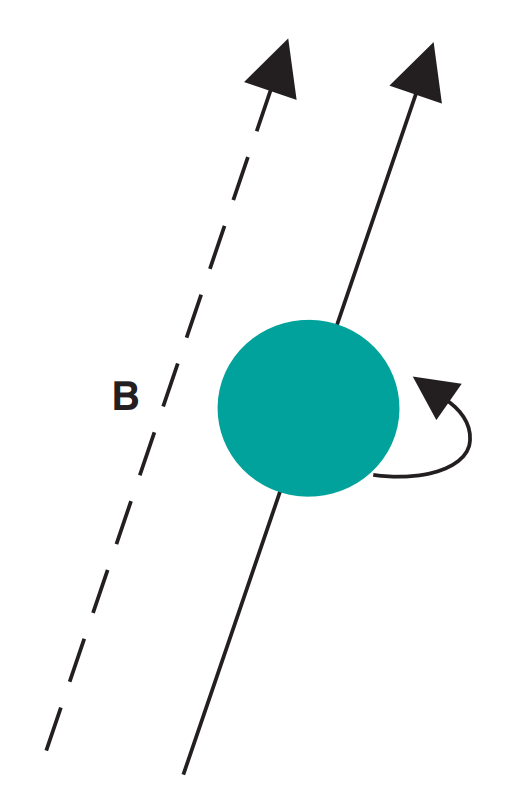
\includegraphics[height=0.3\linewidth]{mychapters/chapter-2/figs/one-spin}
		}{\scriptsize\Doi{10.1002/9781119013068}}
		\label{fig:one-spin}}
		\hspace{0.2\linewidth}
	\subfigure[مغناطیس]{
		\copyrightbox[b]{
			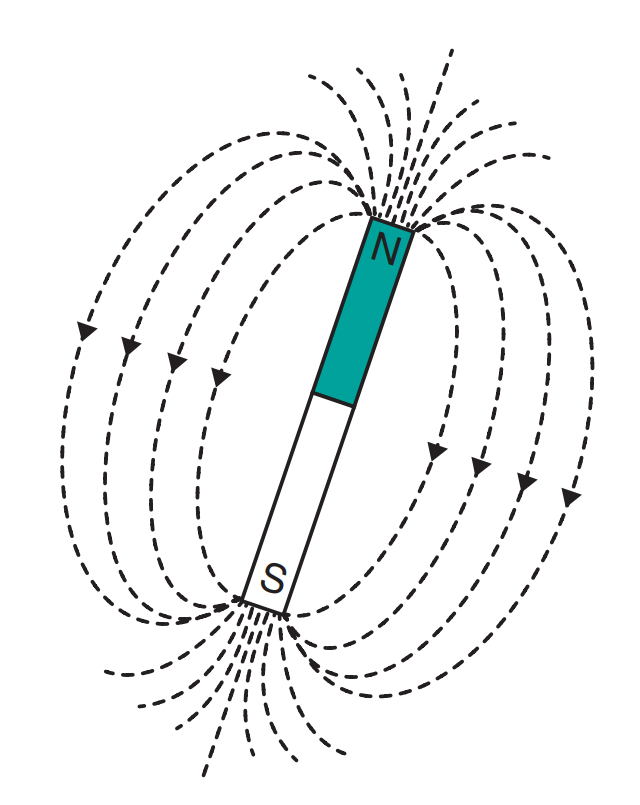
\includegraphics[height=0.3\linewidth]{mychapters/chapter-2/figs/one-magnet}
		}{\scriptsize\Doi{10.1002/9781119013068}}
		\label{fig:one-magnet}}
	\caption{} 
\end{figure}

یکی دیگر از خواص هسته‌ها، اسپین
\index{اسپین}
\LTRfootnote{Spin}
یا اندازه حرکت زاویه ای ذاتی اسپینی
\LTRfootnote{Intrinsic Spin Angular Momentum}
است.
هسته هایی که حرکت اسپینی دارند همواره حول یک محور درحال گردش هستند.(شکل \ref{fig:one-spin} حرکت اسپینی را نمایش می‌دهد.)
تمام عناصر جدول تناوبی
\LTRfootnote{Periodic Table}
بجز آرگون
\LTRfootnote{Argon}
و سریم
\LTRfootnote{Cerium}
حداقل یک ایزوتوپ دارند که حرکت اسپینی دارد. از آنجا که این حرکت نقش مهمی در اصول تصویربرداری \mri دارد، بنابراین تقریبا تمامی عناصر قابلیت مشاهده شدن در تصویربرداری \mri را دارند. اسپین یکی از خواص کوانتومی هسته است و تعداد محدودی اسپین در طبیعت وجود دارند. 

\begin{table}[b]
	\centering
	\begin{tabular}{|C{5em}|C{5em}||C{14em}|}
		\hline \rowcolor{headerColor}
		
		عدد اتمی & جرم اتمی & عدد اسپین
		\\\hline\hline
		زوج & زوج & صفر \\\hline
		فرد & زوج & عدد صحیح \\\hline
		فرد & 
		\multirow{2}{*}{فرد}
		 & 
		\multirow{2}{*}{عدد صحیح و نصفی}
		\\\cline{0-0}
		زوج &  &
		\\\hline
	\end{tabular}
	\caption{بررسی عدد اسپین نسبت به عدد اتمی و جرم اتمی }
	\label{table:spin-even-odd}
\end{table}

\begin{table}[b]
	\centering
	\begin{tabular}{|C{5em}|C{5em}||C{14em}|}
		\hline \rowcolor{headerColor}
		
		تعداد پروتون & تعداد نوترون & عدد اسپین
		\\\hline\hline
		زوج & زوج & صفر \\\hline
		فرد & فرد & عدد صحیح \\\hline
		فرد & زوج & 
		\multirow{2}{*}{عدد صحیح و نصفی}
		\\\cline{0-1}
		زوج & فرد &
		\\\hline
	\end{tabular}
	\caption{بررسی عدد اسپین نسبت به تعداد پروتون‌ها و تعداد نوترون ها }
	\label{table:spin-even-odd-pn}
\end{table}

اسپین که با نماد $I$ و یا $\Phi$ نمایش می‌دهند، مقدایر کوانتیده‌ای به خود می‌گیرد به طوری که می‌تواند صفر یا یک عدد صحیح (مثل $1$و $2$و $3$و ...) و یا یک عدد صحیح و نصفی (مثل $0.5$و $1.5$و $2.5$ و ...) باشد. 
بنابر \cite{book:basic-principles-and-applications}، می‌توان جدول 
\ref{table:spin-even-odd}
را استخراج نمود که آن را می‌توان به شیوه جدول \ref{table:spin-even-odd-pn}
برحسب تعداد پروتون ها و نوترون ها به خاطر سپرد.
درحقیقت اتم‌هایی با عدد اتمی یا جرم اتمی فرد دارای اسپین هستند و اگر هردو زوج باشند، نمی‌توان آن‌ها را در تصویربرداری \mri مطالعه نمود. 

در تصویر برداری \mri ما برروی هسته‌هایی متمرکز هستیم که اسپین آن‌ها \f12 است. به‌طور خاص  در تصویربرداری \mri، هسته اتم هیدروژن
\ce{^1_1H}
(فراوان‌ترین ایزوتوپ هیدروژن) و اتم کربن
\ce{^{13}_6C}
(ایزوتوپ کمیاب اما مفید در تصویربرداری) استفاده می‌شود.\cite{Handouts-NMRhandout.html}
توجه هم داریم که فراوان ترین ایزوتوپ کربن یعنی 
\ce{^{12}_6C}
فاقد اسپین است زیرا تعداد پروتون ها و نوتورون های آن هردو زوج هستند و بنابراین قابل بررسی در تصویربرداری  \mri نیستند. البته اتم های دیگری نیز مانند 
\ce{^19_9F}،
\ce{^23_11Na} و
\ce{^31_15P}
نیز در این تصویربرداری حائز اهمیت می‌باشند.

% READ THIS: http://iverson.cm.utexas.edu/courses/310N/Handouts/NMRhandout.html

اتم هیدروژن 
\ce{^1_1H}
از آن جهت بسیار اهمیت دارد که اولا ساختار بسیار ساده‌ای دارد (هسته آن از یک تک پروتون تشکیل شده است) و ثانیا در ساختمان اصلی آب 
\ce{H2O}
بکار رفته‌اند.
بدن هر‌انسان به طور میانگین، از 60 درصد آب تشکیل شده است. همچنین برخی ارگان های بدن حتی تا 90 درصد از آب ساخته شده‌اند. مغز و قلب انسان 73 درصد آب، ریه ها 83 درصد، پوست 64 درصد، ماهیچه‌ها و کلیه‌ها 79 درصد و استخوان ها 31 درصد آب را شامل می‌شوند.\cite{science-water-you-water-and-human-body}
از این رو، اتم هیدروژن نقش تعیین کننده ای دارد. دقت نیز داریم که اتم اکسیژن \ce{^16_8O} اسپینی ندارد و بنابراین نقشی در تصویربرداری \mri ندارد. از آنجایی که آب در بافت های نرم به میزان بیشتری وجود دارد، این نوع تصویر برداری عموما برای تصویربرداری از نواحی دارای بافت نرم مانند مغز مورد استفاده قرار می‌گیرد.

از آنجایی که درون هسته متشکل از پروتون هاست، بارالکتریکی هسته مثبت است. از این رو، در صورت حرکت دورانی حول محور دوران خود، یک میدان مغناطیسی هم‌راستا با همان محور دوران، ایجاد می‌کند. جون‌که مقدار اندازه اسپین هسته یک مقدار ثابت است این میدان مغناطیسی نیز اندازه ثابتی دارد. بنابراین برای ممان مغناطیسی هسته
\LTRfootnote{Nuclear Magnetic Moment} 
دو مولفه‌ی مقدار و جهت میدان مغناطیسی می‌توان تعریف کرد. به عبارت دیگر یک هسته دارای اسپین را می‌توان به صورت یک آهن‌ربای میکروسکوپیک ریز درنظر گرفت
(شکل \ref{fig:one-magnet}).
برای یک پروتون یا همان هسته ی \ce{^1_1H}، ممان مغناطیسی $\mu$ و تکانه زاویه‌ای اسپینی
\LTRfootnote{Spin Angular Momentum}$\Phi$
با یک ثابت تناسب $\gamma$ به صورت زیر به یک دیگر مرتبط می‌شوند.

\begin{equation}\label{eq:mu=gamma.phi}
	\mu = \gamma . \Phi
\end{equation}

که $\gamma$ در رابطه‌ی بالا نسبت ژایرومغناطیسی 
\LTRfootnote{Gyromagnetic Ratio}
نامیده می‌شود و واحد  $\frac{\gamma}{2\pi}$
را عموما برحسب (\lr{MHz/Tesla})

بیان می‌کنند.



\begin{figure}[t]
	\centering
	\copyrightbox[b]{
		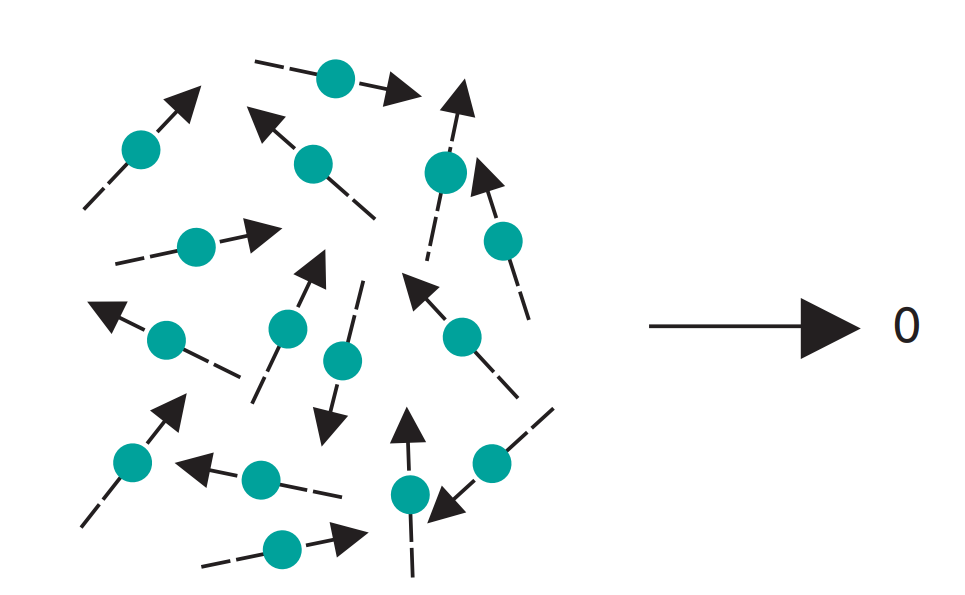
\includegraphics[width=0.5\linewidth]{mychapters/chapter-2/figs/balance-spin}
	}{\scriptsize\Doi{10.1002/9781119013068}}
	\caption{}
	\label{fig:balance-spin}
\end{figure}


در اندازه گیری \mr مجموعه‌ای از این میدان های مغناطیسی کوچک مورد بررسی قرار می‌گیرد و به صورت تکی به قدری نیستند که بتوان آن‌ها را بررسی نمود. جهت این اسپین ها یک مکانیسم تصادفی دارد به طوری که در یک مجموعه هسته داری اسپین، در صورت عدم حضور میدان خارجی، برایند میدان مغناطیسی حاصل در آن مجمموعه صفر است و سیستم درحالت تعادل قرار دارد. 
(شکل \ref{fig:balance-spin}) در واقع تصاویر \mri در ابعاد ماکروسکوپیک ثبت می‌شوند.


\begin{figure}
	\centering
	\copyrightbox[b]{
		\centering
		\begin{minipage}{0.9\linewidth}
				\centering
				\subfigure[]{
				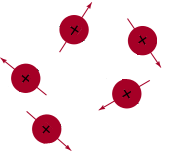
\includegraphics[height=0.25\linewidth]{mychapters/chapter-2/figs/alineamiento-no}	
				\label{subfig:alineamiento-no}}		
				\hspace{0.15\linewidth}
				\subfigure[]{
				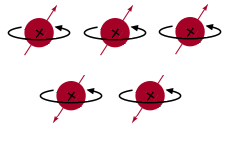
\includegraphics[height=0.22\linewidth]{mychapters/chapter-2/figs/alineamiento-yes}	
				\label{subfig:alineamiento-yes}} 
		\end{minipage}	
	}{\urlSource{http://www.qorganica.es/QOT/T12/alineamiento_e_exported/index.html}}
	\caption{}\label{fig:alineamiento}
\end{figure}



\begin{figure}
	\centering	
	\subfigure[]{
	\copyrightbox[b]{
		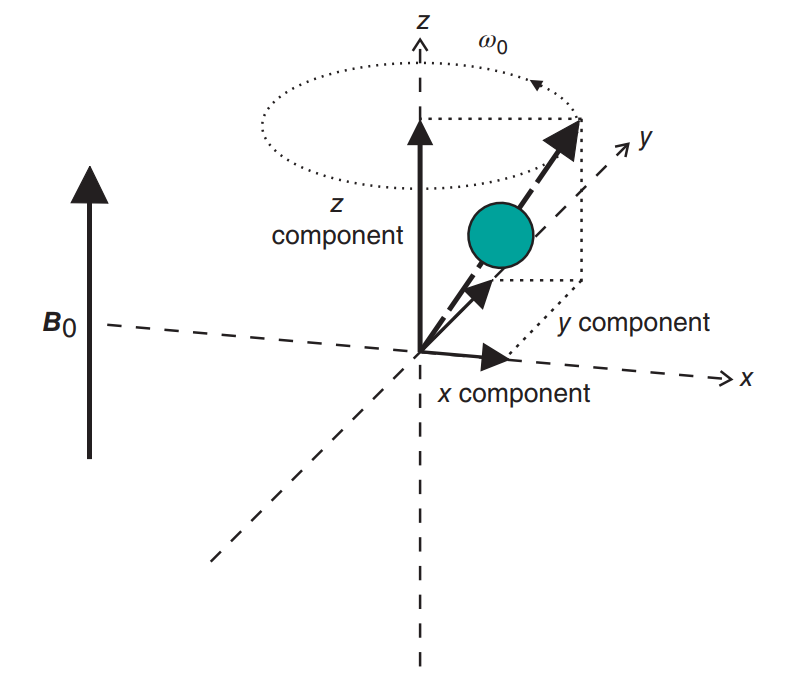
\includegraphics[height=0.35\linewidth]{mychapters/chapter-2/figs/B-spin}	
		\label{subfig:precession-spin}
	}{\scriptsize\Doi{10.1002/9781119013068}}}
	\hspace{0.1\linewidth}
	\subfigure[]{
	\copyrightbox[b]{
		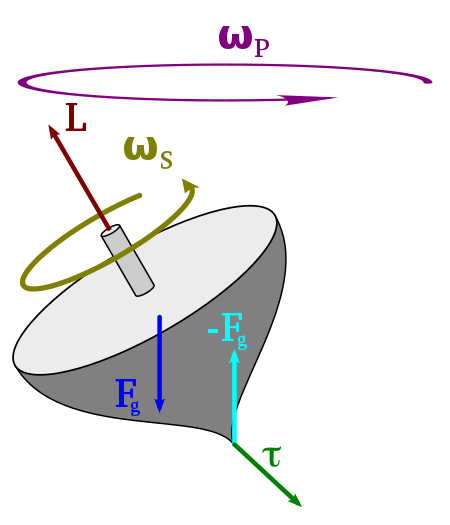
\includegraphics[height=0.3\linewidth]{mychapters/chapter-2/figs/PrecessionOfATop}	
		\label{subfig:precession-top}
	}{\urlSource{https://w.wiki/3TPJ}}}
	\caption{}
	\label{fig:precession}

\end{figure}

\subsubsection{پروتون‌ها در یک میدان مغناطیسی خارجی}


هنگامی که پروتون دارای اسپین در داخل یک \textit{میدان مغناطیسی قوی }
\RTLfootnote{
هنگامی که از میدان مغناطیسی قوی صحبت می‌کنیم منظور چیزی حدود حداقل $1$ تسلا یا $10000$ گاوس است. 
}
خارجی $B_0$ قرار می‌گیرند، اولا ممان های مغناطیسی اتم ها تمایل پیدا می‌کنند که\textit{هم‌جهت} یا \textit{خلاف جهت} 
\LTRfootnote{Parallel or Anti-parallel}
قرار بگیرند (شکل \ref{subfig:alineamiento-yes}
و ثانیا وادار می‌شوند که حرکت چرخشی حول راستای میدان مغناطیسی خارجی داشته باشند که به این پدیده \textbf{حرکت تقدیمی}
\LTRfootnote{Precession}
می‌گویند. 

\begin{figure}
	\centering\copyrightbox[b]{
		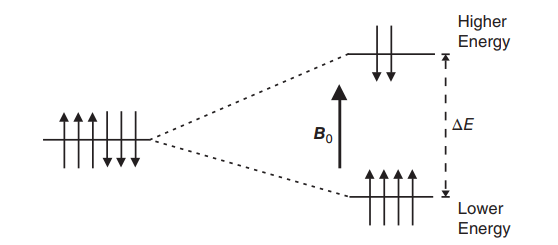
\includegraphics[width=0.6\linewidth]{mychapters/chapter-2/figs/zeeman-diagram}
	}{\scriptsize\Doi{10.1002/9781119013068}}
	\caption{}
	\label{fig:zeeman-diagram}
\end{figure}


همانطور که اشاره شد در اثر یک میدان مغناطیسی خارجی $B_0$ تمایل پیدا می‌کنند که ممان‌های مغناطیسی خود را در جهت یا خلاف جهت آن میدان قرار دهند. آنانی که در جهت آن میدان قرار داشته باشند انرژی کمتر و آنانی که در خلاف جهت آن میدان باشند، انرژی بیشتری را دارا می‌باشند.  تعداد پروتون های زیادی وجود دارند که در جهت و یا خلاف جفت میدان قرار می‌گیرند و تعداد آن ها تقریبا مشابه هم دیگر است که در حقیقت می‌توان گفت اکثر پروتون ها در اثر این میدان  اثر یک دیگر را خنثی می‌کنند اما برایند آن ها صفر نمی‌شود زیرا تعداد آنانی که در جهت میدان قرار می‌گیرند به میزان کمی، بیشتر است که به آن به اصطلاح، \textbf{اسپین اضافه}
\LTRfootnote{Excess Spin}
گفته می‌شود.
(شکل \ref{fig:zeeman-diagram})
از این رو مقدار ناصفری برای \textbf{مغناطیس‌شوندگی شبکه} 
\LTRfootnote{Net Magnitation}
وجود دارد.
به عبارت دقیق‌تر، نسبت 
\RLE{$\frac{\rltext{تعداد هم‌جهت‌ها} - \rltext{تعداد خلاف جهت‌‌ها}}{\rltext{تعداد کل پروتون‌ها}}$}
یک عدد نامنفی بسیار کوچک است. به عنوان مثال، در یک میدان مغناطیسی خارجی $B_0 = 3 \mathrm{T}$ و در دمای اتاق، نسبت مذکور چیزی در حدود $10^{-5}$ می‌باشد. یعنی از یک میلیون پروتونی که در اختیار داریم تنها 10 تای آنان در اسپین اضافه نقش دارند که آن اسپین اضافه در تولید \textbf{سیگنال های \mr}\LTRfootnote{MR Signals}
استفاده می‌شوند.
\begin{figure}
	\centering
	\copyrightbox[b]{
		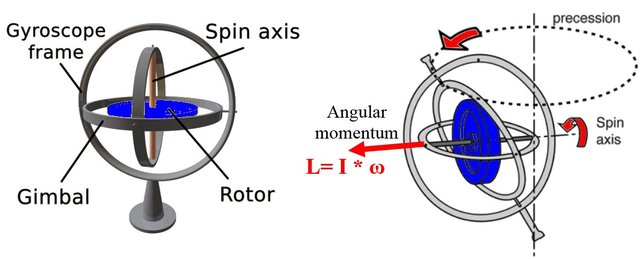
\includegraphics[width=0.7\linewidth]{mychapters/chapter-2/figs/Gyroscope-components}
	}{\urlSource{https://is.gd/T3UkHu}}
	\caption{}
	\label{fig:gyroscope-components}
\end{figure}



پدیده دومی که در اثر قرار گرفتن یک پروتون در درون یک میدان مغناطیسی بسیار قوی برایش اتفاق می‌افتد، حرکت تقدیمی نامیده می‌شود. این پدیده را می‌توان به صورت یک ژایروسکوپ 
(\ref{fig:gyroscope-components})
(شکل \ref{subfig:precession-top}) و یا حرکت آشنای یک فرفره‌ی درحال گردش (شکل \ref{subfig:precession-top})
در نظر گرفت. اگر یک ژیروسکوپ و یا فرفره در راستای عمودی جهت گیری داشته باشد، بدون تلوتلو‌خوردن
\LTRfootnote{Wobbling}
به دور خود می‌چرخد. هنگامی که یک بار محور چرخش ژیروسکوپ از محور عمومی فاصله بگیرد، در اثر میدان مغناطیسی زمین یا همان جاذبه
\LTRfootnote{Gravity}
 شروع به گردش حول محور عمودی خود با فرکانسی مستقل از فرکانس اسپینی مطابق شکل \ref{subfig:precession-top}
می‌کند. 

به‌طور‌خلاصه دو نوع حرکت برای یک پروتون دارای اسپین در یک میدان مغناطیسی قوی می‌توان تصور کرد.

\begin{alphabetlist}
	\item
	حرکت \textbf{اسپینی} هسته به دور محور خود و با فرکانس مخصوص خود که آن حرکت، \textbf{ممان زاویه‌ای اسپینی }را تولید می‌کند و آن نیز باعث ایجاد \textbf{ممان مغناطیسی }می‌شود.
	\item
	حرکت \textbf{تقدیمی} که نوعی تلوتلو خوردن و  گردش حول یک محور دیگه و با فرکانسی مستقل می‌باشد.
\end{alphabetlist}


\subsubsection{مغناطش شبکه}
\textbf{مغناطش شبکه} و یا \textbf{مغناطیس‌شوندگی شبکه} 
\LTRfootnote{Net Magnetization}



\begin{figure}
	\centering
	\copyrightbox[b]{
		\begin{minipage}{0.8\linewidth}\centering
			\subfigure[]{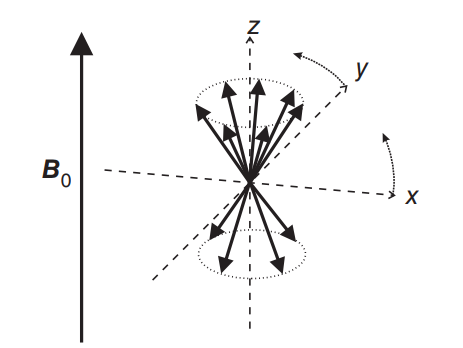
\includegraphics[height=0.3\linewidth]{mychapters/chapter-2/figs/net-mag-a}\label{subfig:net-mag-a}}
			\hspace{0.15\linewidth}
			\subfigure[]{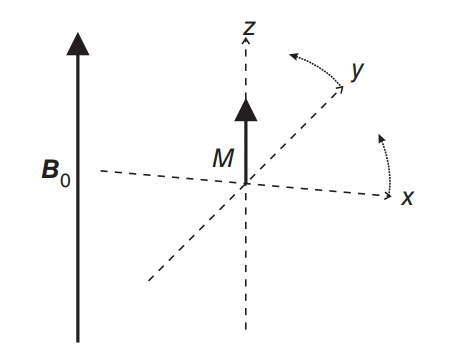
\includegraphics[height=0.3\linewidth]{mychapters/chapter-2/figs/net-mag-b}\label{subfig:net-mag-b}}
		\end{minipage}
	}{\scriptsize\Doi{10.1002/9781119013068}}
	\caption{}
	\label{fig:net-mag}
\end{figure}

موضوع مهم دیگری است که در \mri مطرح می‌شود.
مغناطیس شوندگی هر پروتون را می‌توان به عنوان یک بردار در‌نظر گرفت. مغناطش شبکه را می‌توان به‌عنوان برایند آن بردار ها مطابق شکل \ref{fig:net-mag}در نظر گرفت. 
هر یک از این بردار را می‌توان در راستای میدان به دو مولفه‌ی طولی و عرضی تجزیه نمود. با این مدل‌سازی نیز همان‌طور که پیشتر نیز توضیح داده شد، اکثر مولفه هایی هم‌جهت و خلاف جهت، هم‌دیگر را کنسل می‌کنند و تعداد کمی اسپین های هم‌جهت باقی می‌مانند که اسپین اضافه نام داشتند. اما موله‌عرضی صفر است. جراکه اسپین پروتون‌ها فازی رندم دارند و بنابراین برایند آنان صفر می‌شود. این یعنی مغناطش شبکه، مولفه‌ای در راستای عرضی ندارد و صرفا در راستای مولفه‌ی طولی یا همان راستای میدان مغناطیسی خارجی $B_0$ است (شکل \ref{subfig:net-mag-b})

\subsubsection{فرکانس لامور}

همانند رابطه‌ی بین تکانه زاویه ای اسپینی و ممان مغناطیسی که در رابطه‌ی \ref{eq:mu=gamma.phi} بیان شد، رابطه تناسبی دیگری نیز بین فرکانس زاویه‌ای حرکت تقدیمی $\omega_0$ و میدان مغناطیسی خارجی $B_0$  
با ثابت تناسب ژایرومغناطیسی
\LTRfootnote{Constant Gyromagnetic Ratio}
$\gamma$
وجود دارد:

\begin{equation}
	\omega_0 = \gamma . B_0 \qquad \leftrightarrow \qquad f_0 = \frac{\gamma}{2\pi}. B_0
\end{equation}

عنوان یک مثال، به ازای میدان خارجی $B_0=1 \mathrm{T}$، مقدار $f_0$ برابر $42.58 \mathrm{MHz}$ می‌شود. این فرکانس در شکل \ref{subfig:precession-spin}
نیز نشان داده شده است 
تساوی بالا به‌عنوان \textbf{تساوی لارمور}
\LTRfootnote{Larmor Equation}
شناخته می‌شود و مهم‌ترین معادله ای است که اکثر پدیده‌های مرتبط با \mri را توضیح می‌دهد که از بین آن پدیده‌ها میتوان به رزونانس مغناطیسی و قسمت های تصویر‌برداری مانند مفهوم میدان گرادیان و نقش آن در تصویر‌برداری اشاره نمود.

\begin{table}[b]
	\centering
	\copyrightbox[b]{
	\begin{latin}
		\footnotesize
		\begin{tabularx}{\textwidth}{ | c | c | c | Y | Y | Y | Y | }
			\hline\rowcolor{headerColor}
			Element & Isotope & Spin & Natural Abundance & Quadrupole Moment, Q $(10^{-30} \frac{\mathrm{rad}}{m^2}\mathrm{A})$& Gyromagnetic Ratio $(10^7 \frac{\mathrm{rad}}{Ts})$ & Common Reference Standard\\ \hline\hline
			\multirow{2}{*}{Hydrogen} & \ce{^1H} & \f12 & 100 & 0 & 26.75105 & \ce{Si(CH3)4} \\ \cline{2-7}
			& \ce{^2H} & 1 & < 0.1 & 2.8E-3 & 4.10646 & \ce{Si(CD3)4} \\ \hline
			\multirow{2}{*}{Boron} & \ce{^10B} & 3 & 19.7 & 0.08 & 2.87471 & \ce{BF3.OEt2} \\ \cline{2-7}
			& \ce{^11B} & \f32 & 80.3 & 0.04 & 8.58406 & \ce{BF3.OEt2} \\ \hline
			Carbon & \ce{^13C} & \f12 & 1.1 & 0 & 6.72804 & \ce{Si(CH3)4} \\ \hline
			\multirow{2}{*}{Nitrogen} & \ce{^14N} & 1 & 99.6 & 1 & 1.93297 & \ce{CH3NO2} \\ \cline{2-7}
			& \ce{^15N} & \f12 & 0.4 & 0 & -2.71171 & \ce{CH3NO2} \\ \hline
			Fluorine & \ce{^19F} & \f12 & 100 & 0 & 25.18034 & \ce{CFCl3} \\ \hline
			Aluminium & \ce{^27Al} & \f52 & 100 & 15 & 6.97594 & \ce{Al(NO3)3} in \ce{D2O} \\ \hline
			Silicon & \ce{^29Si} & \f12 & 4.7 & 0 & -5.3146 & \ce{Si(CH3)4} \\ \hline
			Phosphorus & \ce{^31P} & \f12 & 100 & 0 & 10.84015 & 85\% \ce{H3PO4} \\ \hline
			\multirow{2}{*}{Chlorine} & \ce{^35Cl} & \f32 & 75.5 & -7.9 & 2.62401 &\ce{NaCl} in \ce{D2O} \\ \cline{2-7}
			& \ce{^37Cl} & \f32 & 24.5 & -6.2 & 2.18428 & \ce{NaCl} in \ce{D2O} \\ \hline
		\end{tabularx}
	\end{latin}
	}{\urlSource{http://www.acadiau.ca/~bellis/resources/nmr/isotopes.html}}
	\caption{}\label{tab:nmr-common}
\end{table}


\ref{subfig:precession-spin}


\begin{figure}
	\centering
	\copyrightbox[b]{
	\begin{minipage}{\linewidth}\centering
	\subfigure[]{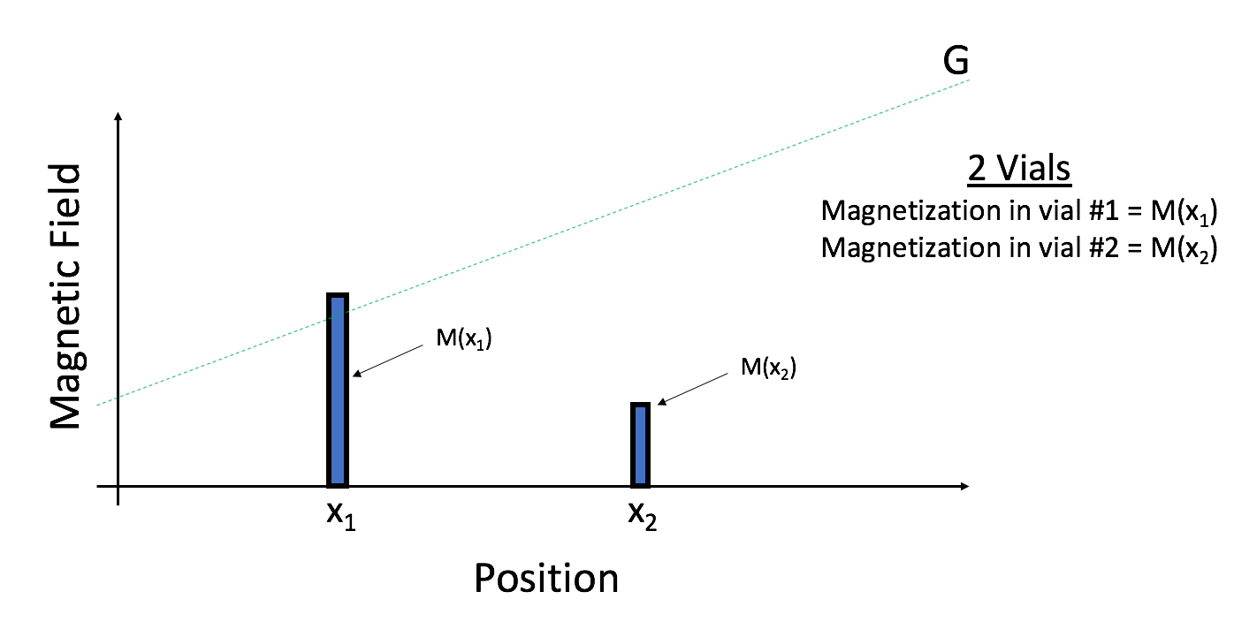
\includegraphics[height=0.23\linewidth]{mychapters/chapter-2/figs/gr-1}\label{subfig:gr1}}
	\hspace{0.08\linewidth}
	\subfigure[]{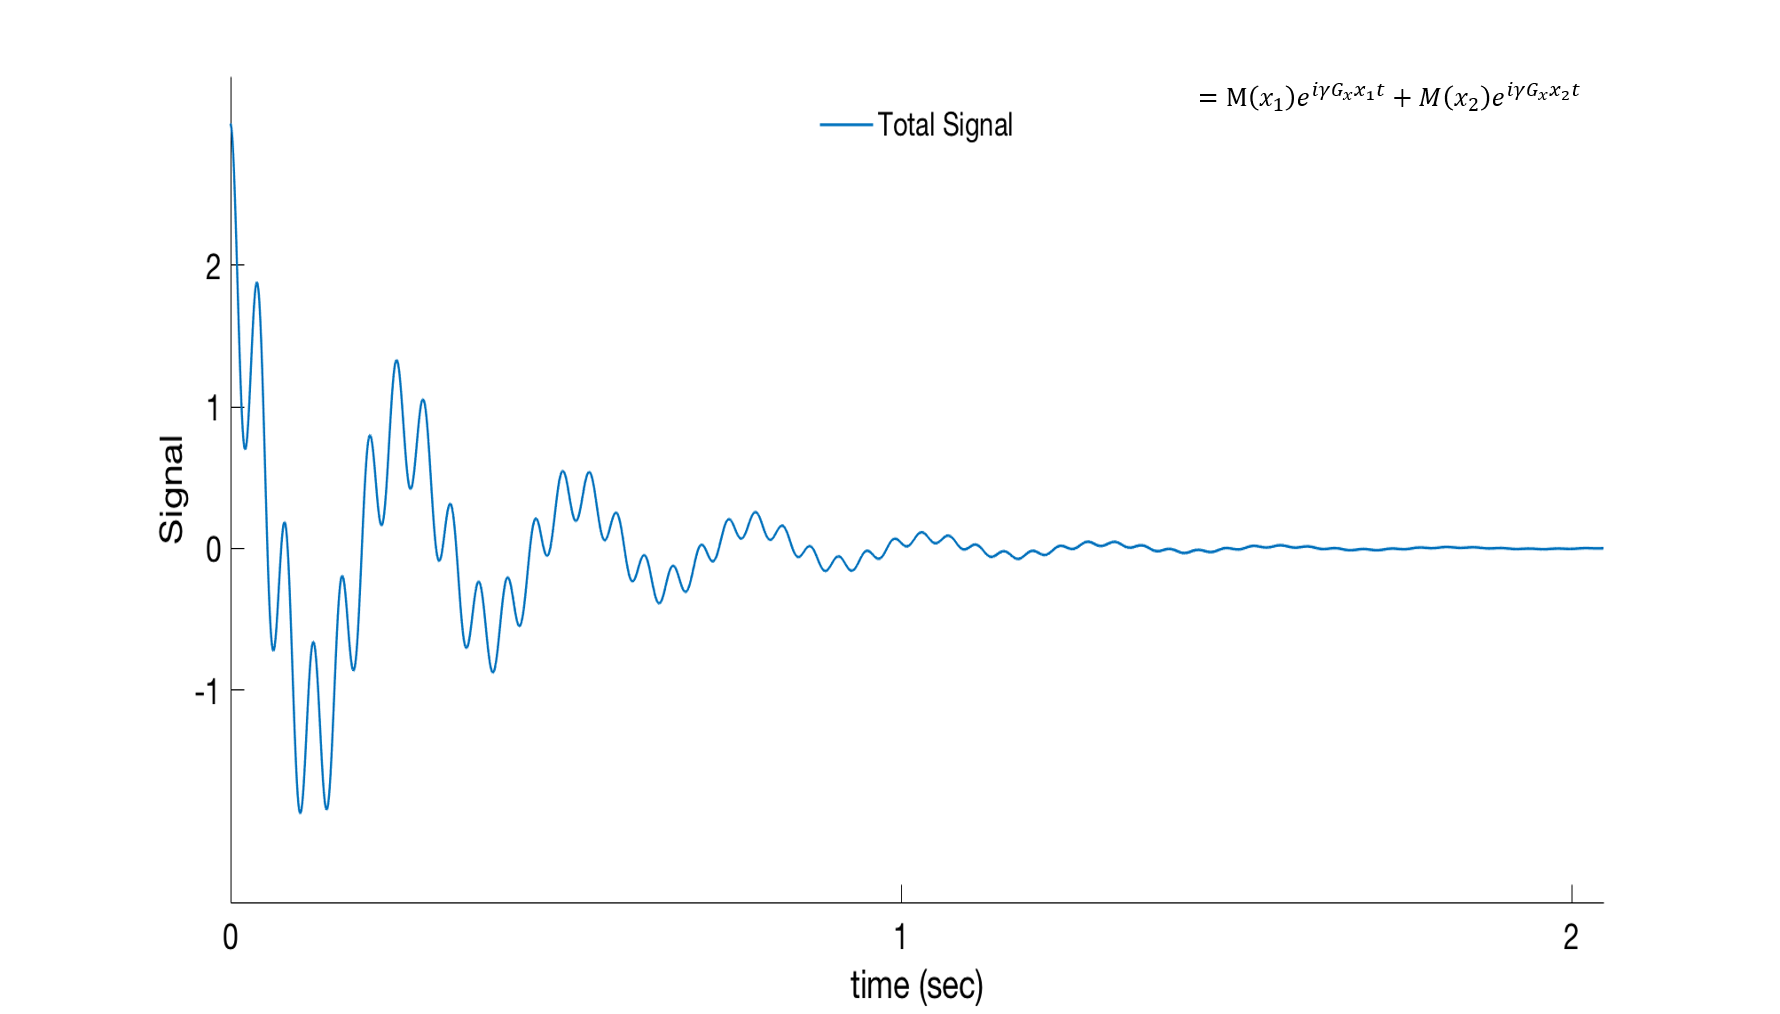
\includegraphics[height=0.23\linewidth]{mychapters/chapter-2/figs/gr-3}\label{subfig:gr3}}
	\subfigure[]{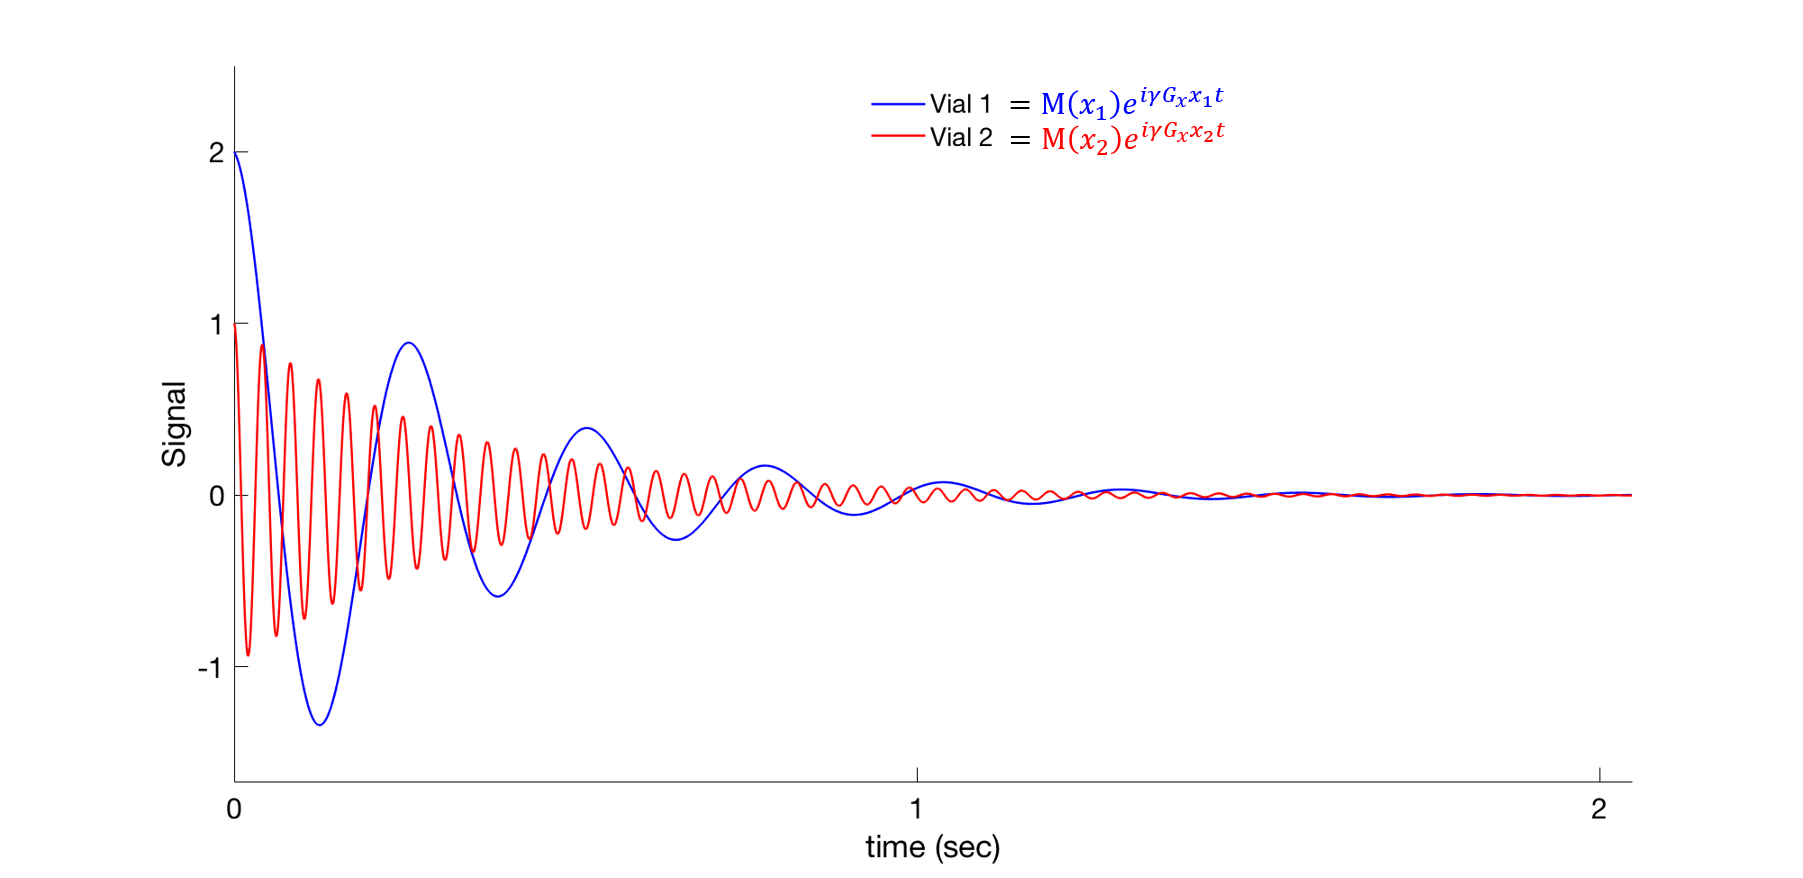
\includegraphics[height=0.23\linewidth]{mychapters/chapter-2/figs/gr-2}\label{subfig:gr2}}
	\hspace{0.08\linewidth}
	\subfigure[]{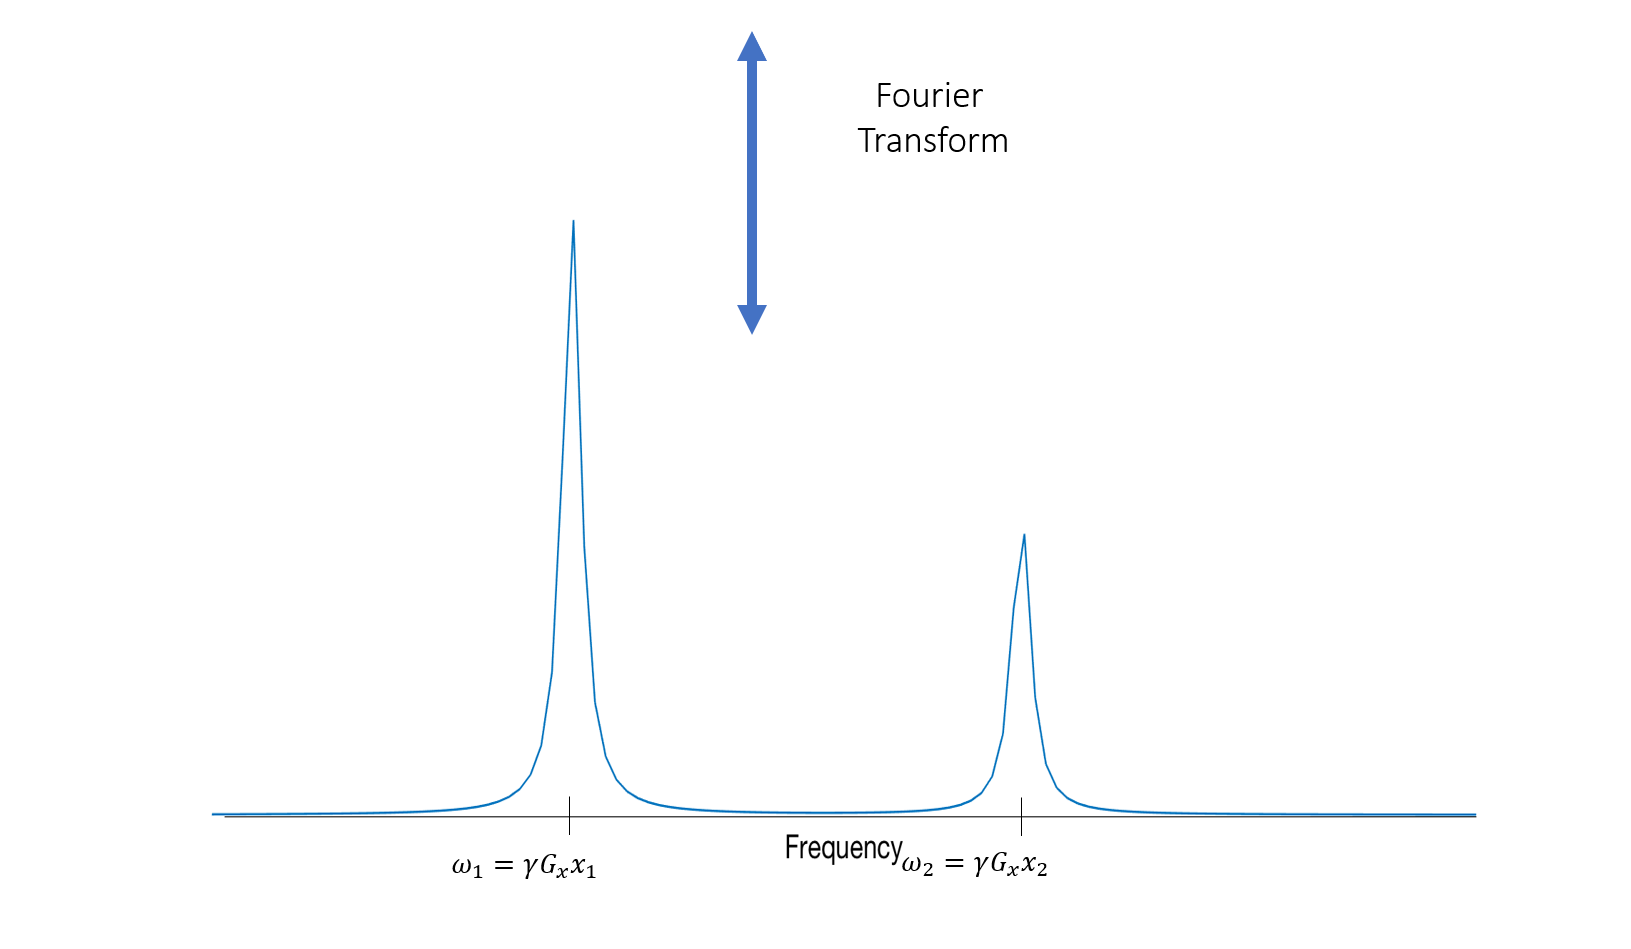
\includegraphics[height=0.25\linewidth]{mychapters/chapter-2/figs/gr-4}\label{subfig:gr4}}
	\end{minipage}
	}{\urlSource{https://yout.be/vC82NeZmL-M}}
	\caption{}
	\label{fig:gr}
\end{figure}



\begin{figure}
	\centering
	\copyrightbox[b]{
		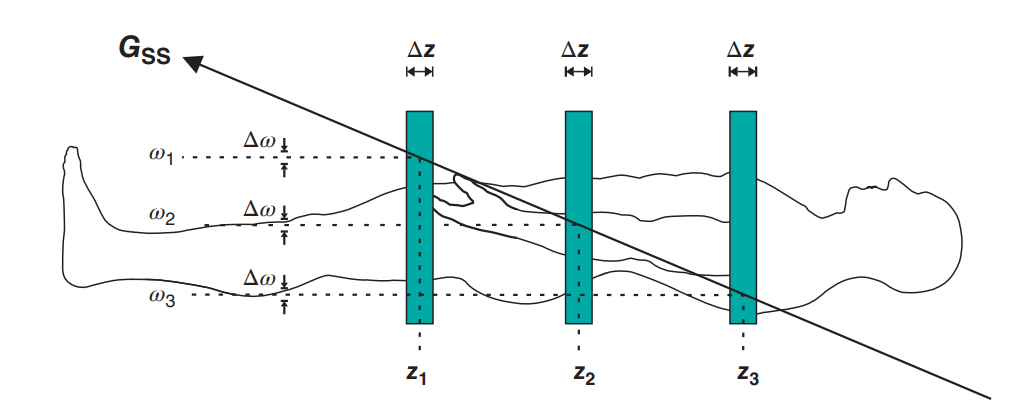
\includegraphics[width=0.7\linewidth]{mychapters/chapter-2/figs/Slice-selection-process}
	}{\scriptsize\Doi{10.1002/9781119013068}}
	\caption{}
	\label{fig:slice-selection-process}
\end{figure}

\begin{figure}
	\centering
	\copyrightbox[b]{
		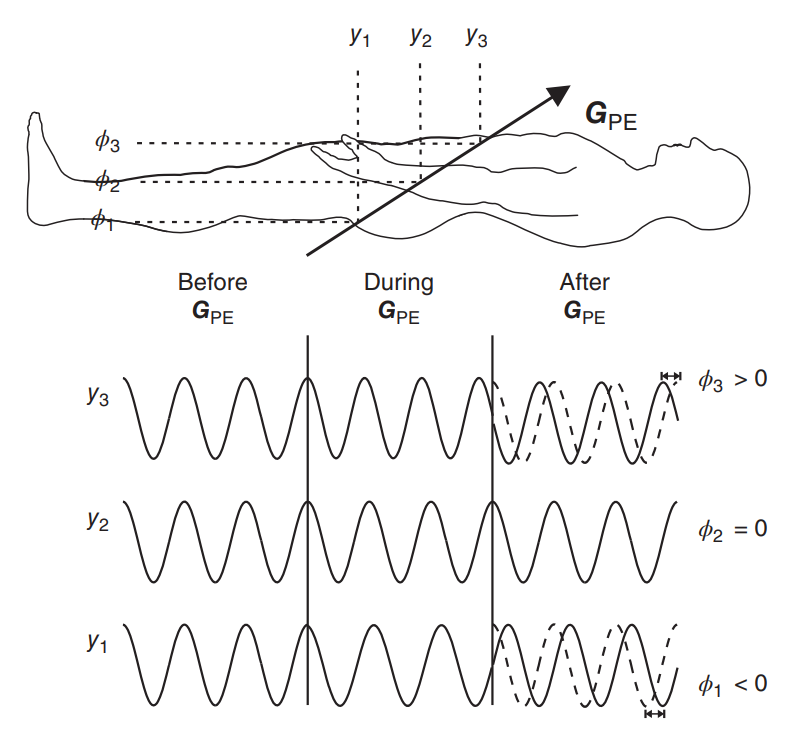
\includegraphics[width=0.7\linewidth]{mychapters/chapter-2/figs/Concept-of-phase-encoding}
	}{\scriptsize\Doi{10.1002/9781119013068}}
	\caption{}
	\label{fig:concept-of-phase-encoding}
\end{figure}













